\chapter {Interfacing LM335, 16x2 LCD display and ESP32}
\thispagestyle{empty}
\label{LCD}
\label{LM335}
\label{ESP32}

\newcommand{\LocTMPfig}{\Origin/user-code/Tmp-Mon/figures}
\newcommand{\LocTMPardcode}{\Origin/user-code/Tmp-Mon/arduino}
\newcommand{\LocTMPardbrief}[1]{{\tt\seqsplit{Origin/user-code/Tmp-Mon/arduino/#1}}}

%%%%%%%%%python
\newcommand{\LocTMPpycode}{\Origin/user-code/Tmp-Mon/python}
\newcommand{\LocTMPpybrief}[1]{{\tt
\seqsplit{Origin/user-code/Tmp-Mon/python/#1}}}
%%%%%%python


This is a Temperature monitoring system that can measure the
room temperature and display the temperature in an LCD display
and also in a webpage by using ESP32 as a webserver. A LM335
temperature sensor is used to measure the temperature. The
output voltage from LM335 is analyzed by Python program and it
calculates the room temperature. This temperature data is sent
to an
LCD display and an ESP32, which in turn sends the temperature
data to a webpage.

UART communication protocol is used in this project. A firmware
code is uploaded into the ESP32 and \arduino\ . \arduino\
responds to various commands send through the Serial port via a
USB-B
cable from the computer. The commands are sent to the Serial
port using Python program.


\section{LM335}
The LM335 temperature sensor is an easy to use, cost-effective
sensor with decent accuracy (around +/- 3 degrees C calibrated).
The sensor is essentially a zener diode whose reverse breakdown
voltage is proportional to absolute temperature.

Since the sensor is a zener diode, a bias current must be
established in order to use the device. The spec sheet states
that the diode should be biased between 400 uA and 5 mA; we'll
bias it
at 1 mA. It is important to note that self-heating can be a
significant factor, which is why we are not choosing a higher
bias current. The bias circuit is as follows:

The temperature sensor's voltage output is related to absolute
temperature by the following equation: \begin{math}Vout = VoutT_{0} *
\frac{T}{T_{0}} \end{math}, where \begin{math}T_{0}\end{math}
is the known reference temperature and \begin{math}
VoutT_{0}\end{math} is the corresponding output voltage. The
nominal \begin{math} VoutT_{0}\end{math} is equal to
\begin{math}T_{0}\end{math} * 10 mV/K. So, at 25 C, \begin{math}
VoutT_{0}\end{math} is nominally 298 K * 10 mV/K = 2.98 V
(to be really accurate, we'd need a reference temperature and a
voltmeter, but nominal values are OK for our purposes). Thus,
the voltage dropped between +5 and the diode is 5V - 2.98V =
2.02V.
In order to get 1 mA bias current, we need a 2.2 K resistor for
R.

\begin{figure}
  \centering
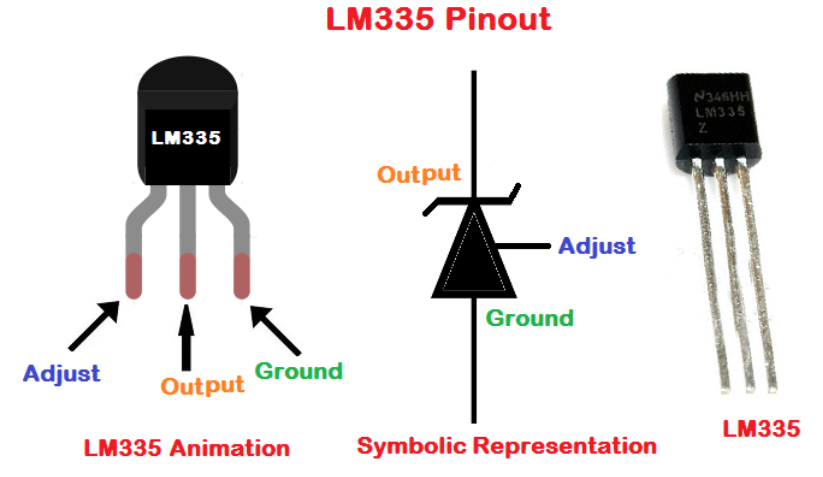
\includegraphics[width=\textwidth]{\LocTMPfig/LM335_pinout.png}  \caption{LM335 pinout}
  \label{fig:lm335pinout}
\end{figure}

\begin{figure}
  \centering
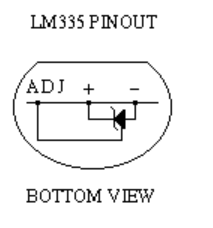
\includegraphics[width=\smfig]{\LocTMPfig/LM335_Schematic.png}  \caption{LM335 Circuit Schematic}
  \label{fig:lm335schematic}
\end{figure}

Note that the adj pin is unconnected. The adj pin is used to
trim the diode to be more accurate. A typical LM335 sensor and
its symbolic representation are shown in the above figure. This
LM335 is connected to the analog pin {\tt A5} of the Arduino Uno
board. The analog voltage, corresponding to the voltage drop,
across the terminals of LM335 needs to be digitized before being
sent to the computer. This is taken care of by an onboard Analog
to Digital Converter (ADC) of ATmega328 microcontroller on the
Arduino Uno board. ATmega328 has a 6-channel, 0 through 5,
10-bit ADC. Analog pin {\tt A5} of the Arduino Uno board, to
which the LM335 is connected, corresponds to channel 5 of the
ADC. As there are 10 bits, 0-5V readings from LM335 are mapped
to the
ADC values from 0 to 1023. LM335 is a commonly available sensor
in the market. It costs about Rs. 70.

\subsection{Interfacing LM335 through the Arduino IDE:}
In this section, we shall describe how to read the voltage
values from a LM335 connected to the analog pin {\tt A5} of the
Arduino Uno board. The LM335 has to be connected to the Arduino
Uno
board before doing these experiments and the Arduino Uno needs
to be connected to the computer with a USB cable, as shown in
\figref{fig:ard-lm335}. Then run the code given in
\ardref{ard:lm335} using Arduino IDE.

\begin{figure}
  \centering
  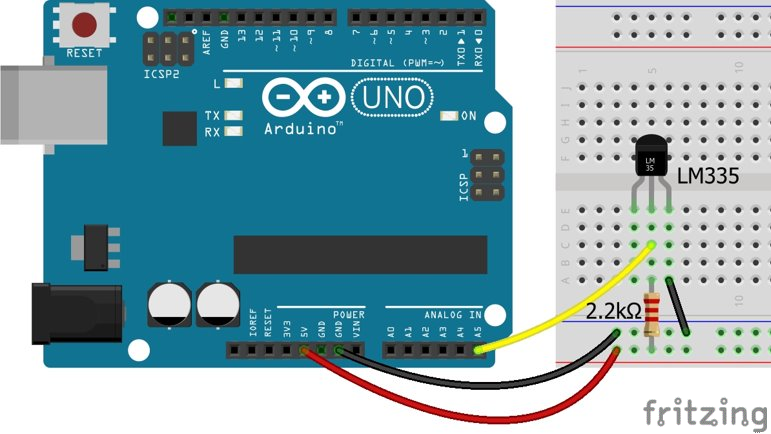
\includegraphics[width=\textwidth]{\LocTMPfig/LM335.png}
  \caption{LM335 and \arduino\ connected using a breadboard}
  \label{fig:ard-lm335}
\end{figure}

\begin{enumerate}
\item As discussed earlier, the 0-5V LM335 readings are mapped
to 0-1023 through an ADC. The Arduino IDE based command for the
analog read functionality is given by
\lstinputlisting[firstline=8,lastline=8]{\LocTMPardcode/LM335/LM335.ino}
where {\tt A5} represents the analog pin 5 to be read and the
read LDR values are stored in the variable {\tt val}.

\item The output voltage from LM335 increases by 10mV per degree
Celsius increase in temperature.
Hence the conversion of the Analog input to temperature in
Celsius is given below.
\lstinputlisting[firstline=9,lastline=9]{\LocTMPardcode/LM335/LM335.ino}

\item The read values are then displayed in {\tt Serial Monitor}
using the code given below,
\lstinputlisting[firstline=10,lastline=10]{\LocTMPardcode/LM335/LM335.ino}

\item The delay in the code is added so that the readings do not
scroll away very fast.
\lstinputlisting[firstline=11,lastline=11]{\LocTMPardcode/LM335/LM335.ino}      
\end{enumerate}

\begin{ardcode}
  \acaption{To Read and display the output from LM335}
  {To Read and display the output from LM335.  Available at
    \LocTMPardbrief{LM335/LM335.ino}.}
  \label{ard:lm335}
  \lstinputlisting{\LocTMPardcode/LM335/LM335.ino}
\end{ardcode}

\subsection{Interfacing LM335 through Python}
In this section, we shall describe how to read the voltage
values from a LM335 connected to the analog pin {\tt A5} of the
Arduino Uno board using Python. The firmware code given should
be
uploaded to the Arduino board. The LM335 has to be connected to
the Arduino Uno board before doing these experiments and the
Arduino Uno needs to be connected to the computer with a USB
cable,
as shown in \figref{fig:ard-lm335}. After doing all the above,
run the \pyref{py:lm335}.

\begin{enumerate}
  \item Declare the pins used for the LM335 using a variable.
\lstinputlisting[firstline=24,lastline=24]
        {\LocTMPpycode/TMP-mon.py}.
        
\item The Python based command for the analog read functionality
is given by,
\lstinputlisting[firstline=35,lastline=35]
        {\LocTMPpycode/TMP-mon.py}

\item The input values are converted as shown in the previous
section
\lstinputlisting[firstline=36,lastline=37]
        {\LocTMPpycode/TMP-mon.py} and printed ,
\lstinputlisting[firstline=45,lastline=46]
        {\LocTMPpycode/TMP-mon.py}
\end{enumerate}

\begin{figure}[htp]
  \centering
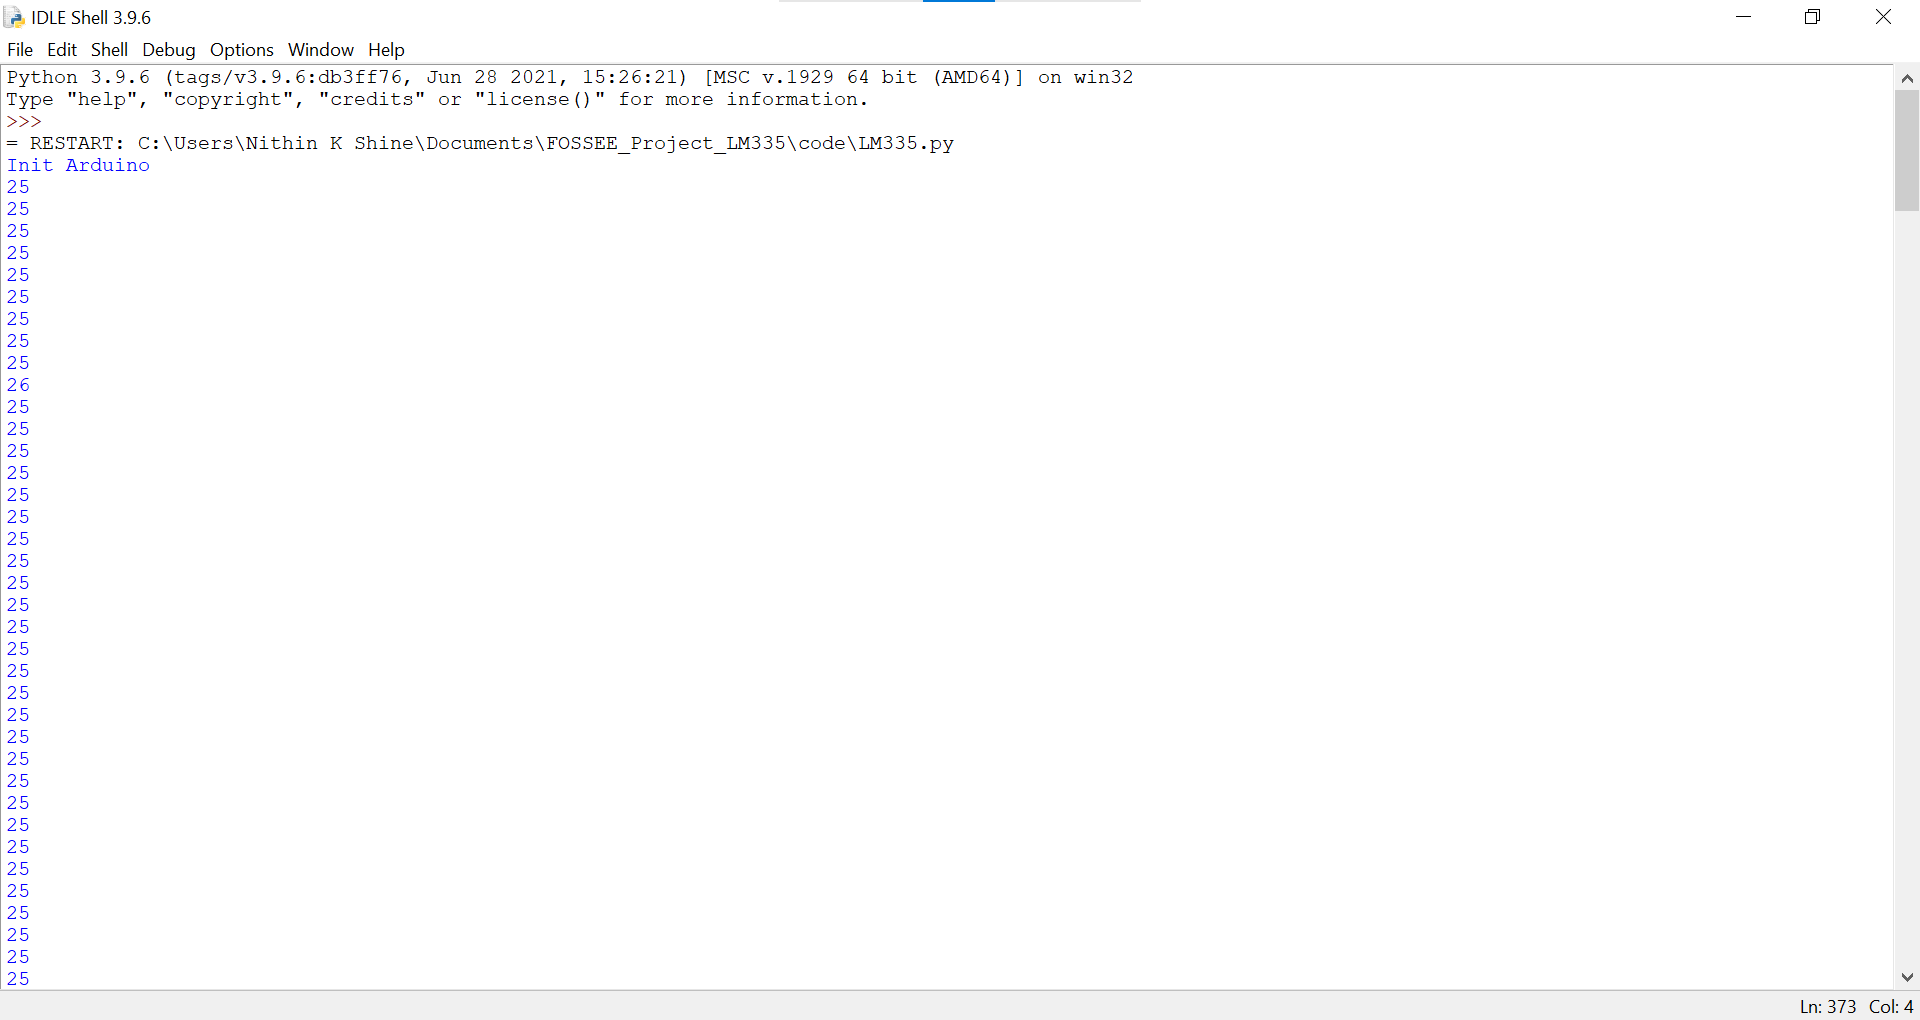
\includegraphics[width=\textwidth]{\LocTMPfig/python-idle.png}  \caption{Temperature display in Python IDLE}
\end{figure}

\begin{pycode}
  \pcaption{To Read and display the output from LM335}
  {To Read and display the output from LM335. Available at
    \LocTMPpybrief{TMP-mon.py}.}
  \label{py:lm335}
  \lstinputlisting{\LocTMPpycode/TMP-mon.py}
\end{pycode}


\section{LCD display}
The Liquid Crystal Display has a parallel interface. It means
that the microcontroller operates several pins at once to
control the LCD display.
The 16-pins present on the LCD display are discussed below:

\begin{figure}
  \centering
  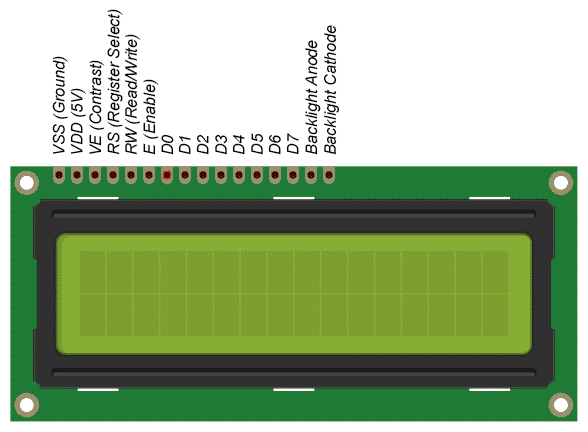
\includegraphics[width=\textwidth]{\LocTMPfig/LCD-pin.png}
  \caption{LCD pinout}
  \label{fig:LCDpinout}
\end{figure}

\begin{itemize}
\item\textit{Contrast Select (VEE): }Pin3 will connect with
power and ground through 3 pin potentiometers. It will help to
control the contrast of PIXELS according to the 16X2 LCD light.
10K
ohm variable resistor is connected with the VEE pin to adjust
light contrast. Variable resistor's one side is connected with 5
volts and the other side is connected with ground. The third
terminal is connected with the VEE pin.
\item\textit{RS: }The Register Select (RS) pin controls the
memory of the LCD in which we write the data. We can select
either the data register or the instruction register. The LCD
looks for
the upcoming instruction, which is present in the instruction
register.
\item\textit{R/W: }The Read/Write pin selects the reading or
writing mode.
\item\textit{E: }The Enable (E) mode is used to enable the
writing to the registers. It sends the data to the data pins
when the mode is HIGH.
\item\textit{D0 to D7: }These are eight data pins numbered as
D0, D1, D3, D3, D4, D5, D6, and D7. We can set the state of the
data pin either HIGH or LOW.
\item\textit{VSS: }It’s a ground pin for common grounds.
\item\textit{VDD: }The power pin will use for voltage input to
the 16X2 LCD.
\item\textit{Backlight Anode and Backlight Cathode: }These pins
are used to power the backlight LED. They are connected to the
5V through a 220-ohm resistor and to the ground respectively.
\end{itemize}

There are two modes of operation for LCD:4-bit mode and 8-bit
mode
\begin{itemize}
\item 8-bit mode: 8 bits of a byte are sent at the same time in
pin DO to D7.
\item 4-bit mode: 8 bits of a byte is sent two times, each time
4 bits in pin D4 to D7.
\end{itemize}
8-bit mode is faster than the 4-bit mode, but use more pins than
4-bit mode. The mode selection is performed at the
initialization process by sending a command to LCD.
This project uses 4-bit mode, which is the most common-used.

In this mode, LCD's pins are connected as follows:
\begin{itemize}
\item 6 pins (RS, EN, D4, D5, D6, and D7) are connected to
Arduino's pin.
\item 4 pins (DO, DI, D2, and D3) are NOT connected.
\item 6 remaining pins are connected to GND/VCC or
potentiometer.
\end{itemize}

LCD Coordinate: LCD 16x2 includes 16 columns and 2 rows. the
columns and rows are indexed from 0.
\begin{figure}
  \centering
  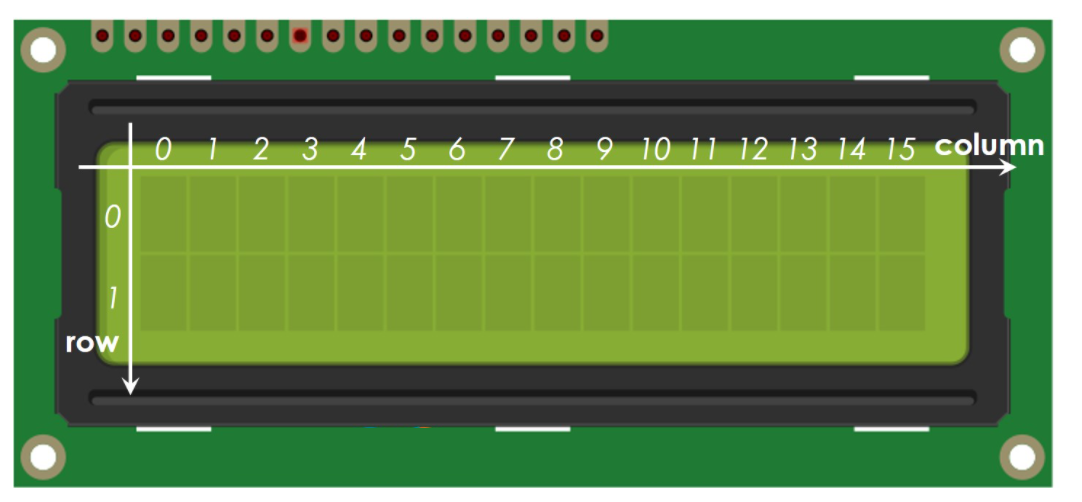
\includegraphics[width=\textwidth]{\LocTMPfig/LCD-pos.png}
  \caption{LCD Coordinates}
  \label{fig:LCD-pos}
\end{figure}

The process of sending data (to be displayed) to LCD:
\begin{enumerate}
\item Arduino sets RS pin to HIGH (to select data register)
\item Arduino writes data to D4 - D7 pins (data bus).
\item LCD receives data on the data bus.
\item LCD stores the received data in the data resistor since
the RS pin is HIGH. Then, LCD displays the data on the screen.
\end{enumerate}

\begin{figure}
  \centering
  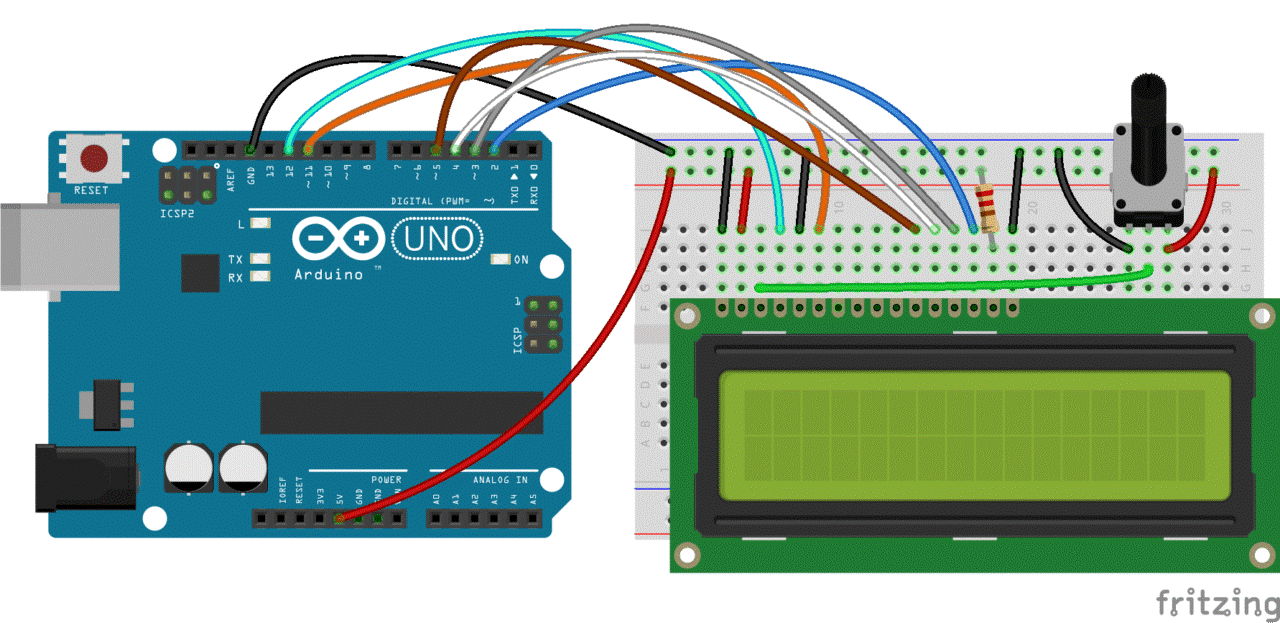
\includegraphics[width=\textwidth]{\LocTMPfig/LCD.png}
  \caption{LCD and \arduino\ connected using a breadboard}
  \label{fig:ard-lcd}
\end{figure}

\subsection{Interfacing LCD display through the Arduino IDE:}
Controlling LCD is a quite complicated task. Fortunately, thanks
to the LiquidCrystal library, this library simplifies the
process of controlling LCD for you so we don't need to know the
low-level instructions. We just need to connect Arduino to LCD
as shown in \figref{fig:ard-lcd} and use the functions of the
library.

\begin{enumerate}
  \item Include the library: 
\lstinputlisting[firstline=1,lastline=1]{\LocTMPardcode/LCD/LCD.ino}
\item Define which Arduino's pin connected to six LCD's pins:
{\tt RS}, {\tt EN}, {\tt D4}, {\tt D5}, {\tt D6}, {\tt D7}
\lstinputlisting[firstline=2,lastline=2]{\LocTMPardcode/LCD/LCD.ino}
\item Declare a LiquidCrystal object,
\lstinputlisting[firstline=3,lastline=3]{\LocTMPardcode/LCD/LCD.ino}
\item Set up the LCD's number of columns and rows.
\lstinputlisting[firstline=7,lastline=7]{\LocTMPardcode/LCD/LCD.ino}
\item Move cursor to the desired position,
\lstinputlisting[firstline=8,lastline=8]{\LocTMPardcode/LCD/LCD.ino}
\item Print a message to the LCD.
\lstinputlisting[firstline=9,lastline=9]{\LocTMPardcode/LCD/LCD.ino}
\end{enumerate}

\begin{ardcode}
  \acaption{To display a string in LCD}
  {To display a string in LCD.  Available at
    \LocTMPardbrief{LCD/LCD.ino}.}
  \label{ard:lcd}
  \lstinputlisting{\LocTMPardcode/LCD/LCD.ino}
\end{ardcode}

\subsection{Interfacing LCD display through Python}
In this section, we discuss how to carry out the experiments of
the previous section from Python. We will list the same
experiment. The LCD should be attached to the Arduino Uno board
before
doing these experiments and the Arduino Uno needs to be
connected to the computer with a USB cable, as shown in
\figref{fig:ard-lcd}. The firmware code should be uploaded to
the Arduino board.
After doing all the above, run the code given in \pyref{py:lcd}.
\begin{enumerate}
  \item Declare the pins used for the LCD using a variable.
        \lstinputlisting[firstline=25,lastline=30]
        {\LocTMPpycode/TMP-mon.py} 

  \item The python-based command to print the string in LCD is,
\lstinputlisting[firstline=41,lastline=41]
        {\LocTMPpycode/TMP-mon.py} 
\end{enumerate}

\begin{pycode}
  \pcaption{To display a string in LCD}
  {To display a string in LCD. Available at
    \LocTMPpybrief{TMP-mon.py}.}
  \label{py:lcd}
  \lstinputlisting{\LocTMPpycode/TMP-mon.py}
\end{pycode}

\section{ESP32}
ESP32 is a low-cost System on Chip (SoC) Microcontroller from
Espressif Systems, the developers of the famous ESP8266 SoC. It
is a successor to ESP8266 SoC and comes in both single-core and
dual-core variations of the Tensilica’s 32-bit Xtensa LX6
Microprocessor with integrated Wi-Fi and Bluetooth.

ESP32 has an integrated RF components like Power Amplifier,
Low-Noise Receive Amplifier, Antenna Switch, Filters and RF
Balun. This makes designing hardware around ESP32 very easy as
we
require very few external components. Designing battery operated
applications like wearables, audio equipment, baby monitors,
smart watches, etc., using ESP32 is very easy.

\begin{figure}
  \centering
  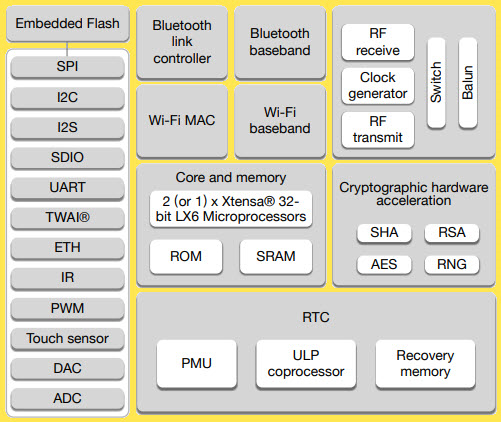
\includegraphics[width=\textwidth]{\LocTMPfig/ESP-block.png}
  \caption{ESP32-Block-Diagram}
  \label{fig:ESPblock}
\end{figure}

Specifications:
\begin{itemize}
\item Single or Dual-Core 32-bit LX6 Microprocessor with clock
frequency up to 240 MHz.
\item 520 KB of SRAM, 448 KB of ROM and 16 KB of RTC SRAM.
\item Supports 802.11 b/g/n Wi-Fi connectivity with speeds up to
150 Mbps.
\item Support for both Classic Bluetooth v4.2 and BLE
specifications.
\item 34 Programmable GPIOs.
\item Up to 18 channels of 12-bit SAR ADC and 2 channels of
8-bit DAC
\item Serial Connectivity include 4 x SPI, 2 x I2C, 2 x I2S, 3 x
UART.
\item Ethernet MAC for physical LAN Communication (requires
external PHY).
\item 1 Host controller for SD/SDIO/MMC and 1 Slave controller
for SDIO/SPI.
\item Motor PWM and up to 16-channels of LED PWM.
\item Secure Boot and Flash Encryption.
\item Cryptographic Hardware Acceleration for AES, Hash (SHA-2),
RSA, ECC and RNG.
\end{itemize}
Espressif Systems released several modules based on ESP32 and
one of the popular options is the ESP-WROOM-32 Module. It
consists of ESP32 SoC, a 40 MHz crystal oscillator, 4 MB Flash
IC and
some passive components.

The ESP32 DevKit Board contains the ESP-WROOM-32 as the main
module and also some additional hardware to easily program ESP32
and make connections with the GPIO Pins.

\begin{figure}
  \centering
  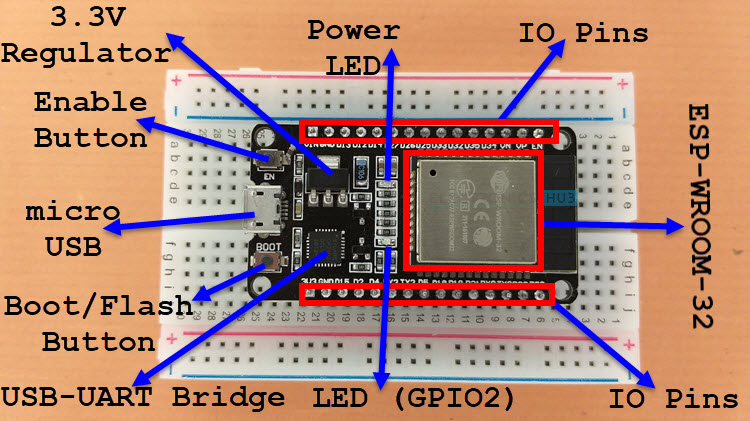
\includegraphics[width=\smfig]{\LocTMPfig/ESP-layout.png}
  \caption{ESP32 DevKit Board Layout}
  \label{fig:ESPlayout}
\end{figure}

\begin{figure}
  \centering
  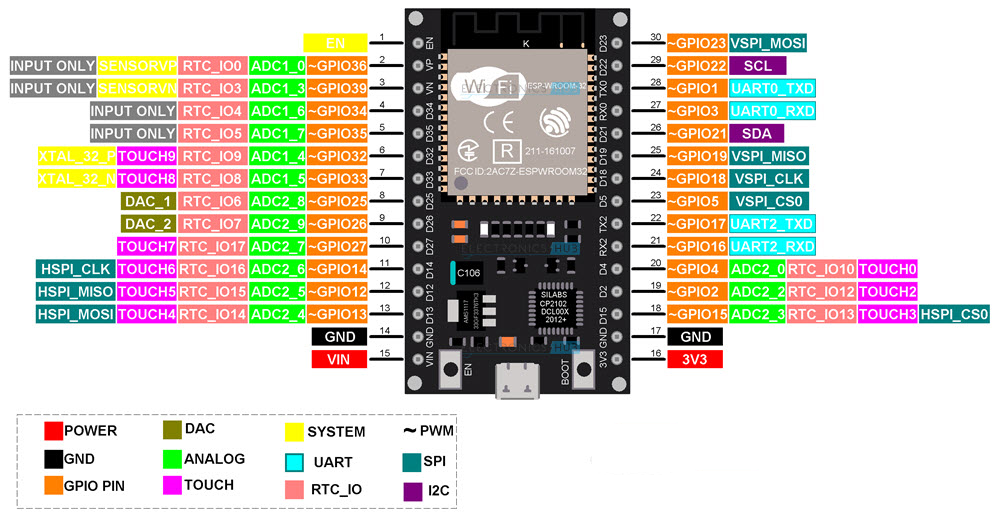
\includegraphics[width=\textwidth]{\LocTMPfig/ESP-pinout.png}
  \caption{ESP32 pinout}
  \label{fig:ESPpinout}
\end{figure}

\subsection{UART communication between Arduino Uno and ESP32:}
In this project I have read some data from Arduino Uno using
ESP32 serially using UART communication protocol. To do this
first we need to connect both the boards serially. Challenge
over here
is that our ESP32 board works on 3.3V whereas Arduino Uno works
on 5V. To establish a proper communication channel between the
two it is required to bring the voltage of Arduino board to
3.3V.
To achieve this, I have made a voltage divider circuit using two
10k resistors. As shown in \figref{fig:ard-uart}

\begin{figure}
  \centering
  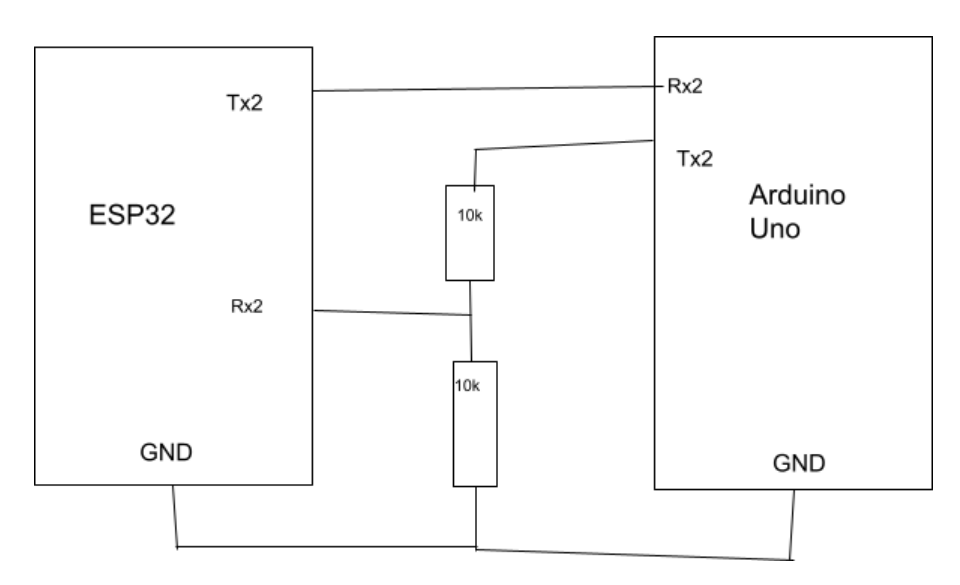
\includegraphics[width=\smfig]{\LocTMPfig/ESP-uart.png}
  \caption{Arduino-ESP32 UART-Circuit schematic}
  \label{fig:ard-uart}
\end{figure}

\begin{figure}
  \centering
  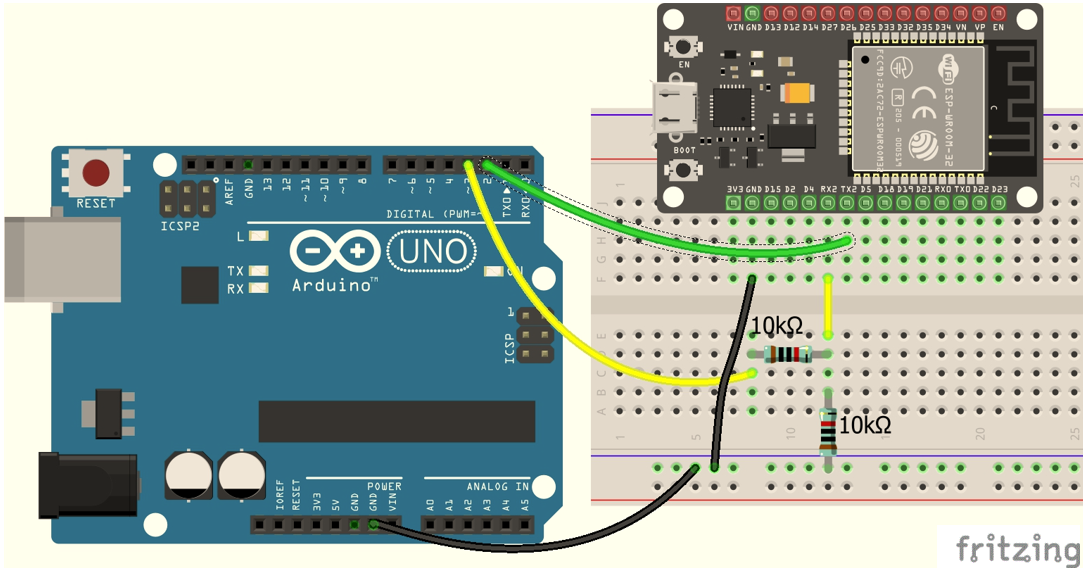
\includegraphics[width=\textwidth]{\LocTMPfig/ESP.png}
  \caption{Arduino-ESP32 UART connection using breadboard}
  \label{fig:ESP}
\end{figure}

\subsection{Interfacing ESP32 through the Arduino IDE}
To print a string in a {\tt website} from ESP32, we should
connect the ESP32 to a Wi-Fi network. Then using the functions
available in Arduino IDE and following the HTTPS protocol we can
print
any string in an IP address, which can easily be accessed by any
devices connected to the same network. The code for this is
given below, \ardref{esp:uart} is to be uploaded to the ESP32
and
\ardref{ard:uart} is to be uploaded to Arduino Uno. The circuit
is given in \figref{fig:ESP}

\begin{enumerate}
\item The string {\tt st} is received from Arduino through UART communication protocol and is send to a website using the functions available in WiFi.h library
        \lstinputlisting[firstline=58,lastline=58]
        {\LocTMPardcode/esp-uart/esp-uart.ino} 
        
\item The string is followed by a line break,
\lstinputlisting[firstline=59,lastline=59]
        {\LocTMPardcode/esp-uart/esp-uart.ino}
\end{enumerate}

\begin{ardcode}
\acaption{To read and display a string sent by Arduino Uno in a website
(UART communication)}
{Uploaded to ESP32 to read and display the value sent by Arduino
Uno(through UART protocol) in a webpage. Available at
    \LocTMPardbrief{esp-uart/esp-uart.ino}.}
  \label{esp:uart}
  \lstinputlisting{\LocTMPardcode/esp-uart/esp-uart.ino}
\end{ardcode}

\begin{ardcode}
  \acaption{To send data to ESP32 (UART communication)}
{Uploaded to Arduino to Sent data to ESP32 through UART
protocol. Available at
    \LocTMPardbrief{ard-uart/ard-uart.ino}.}
  \label{ard:uart}
  \lstinputlisting{\LocTMPardcode/ard-uart/ard-uart.ino}
\end{ardcode}

\subsection{Interfacing ESP32 through Python}
In this section, we discuss how to send a string to a webpage
using ESP32 from Python. The ESP32 should be connected to the
Arduino Uno board (as in \figref{fig:ESP}) before doing these
experiments and the Arduino Uno needs to be connected to the
computer with a USB cable. Give the SSID and password of the
Wi-Fi network in the ESP32 firmware code. The Firmware code
should be
uploaded to the Arduino board and the ESP32. Note down the IP
address from the Serial port of ESP32, which is usually same
every time, when connected to the same Wi-Fi network. The blue
light
of ESP32 glows when its successfully connected to the Wi-Fi
network. In case the LED doesn’t glow press the EN(restart)
button on the ESP32 and wait for 5 seconds. After doing all the
above,
run the \pyref{py:esp}.

\begin{enumerate}
\item Declare the pins used for the Rx and Tx using a variable, \lstinputlisting[firstline=31,lastline=32]
        {\LocTMPpycode/TMP-mon.py} 
        
\item The python-based command to print the string st in webpage
is,
\lstinputlisting[firstline=44,lastline=44]
{\LocTMPpycode/TMP-mon.py} 
\item Finally open the IP address obtained from the ESP32 Serial
port on any device connected to the same Wi-Fi network to view
the temperature.
\end{enumerate}

\begin{pycode}
  \pcaption{To Send a string to a website}
  {To Send a string to a website. Available at
    \LocTMPpybrief{TMP-mon.py}.}
  \label{py:esp}
  \lstinputlisting{\LocTMPpycode/TMP-mon.py}
\end{pycode}

\begin{figure}
  \centering
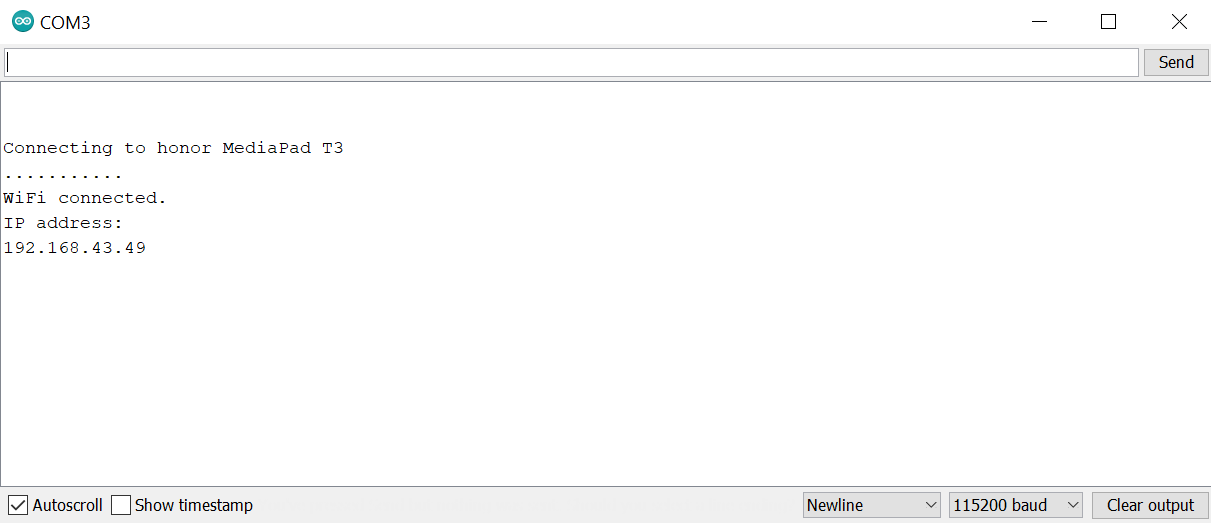
\includegraphics[width=\textwidth]{\LocTMPfig/ESP32-Serial.png}  \caption{ESP-32 Serial port}
\end{figure}

\begin{figure}
  \centering
  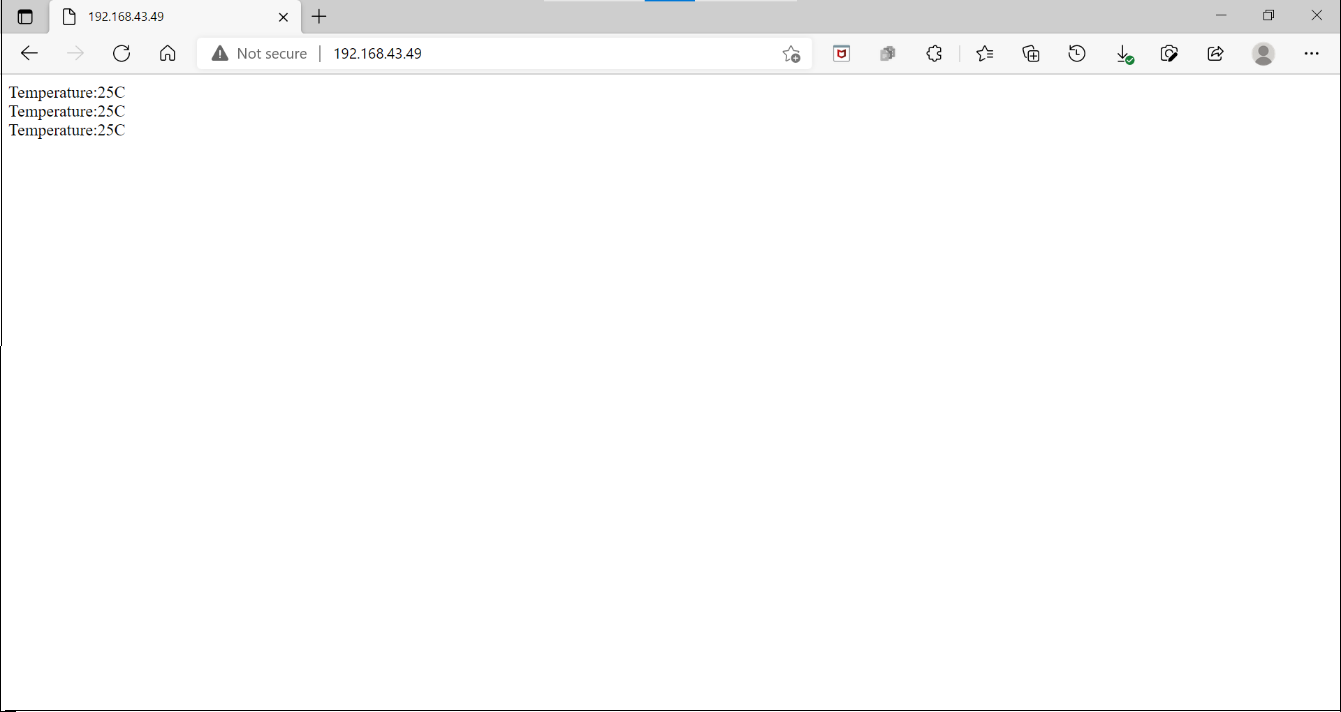
\includegraphics[width=\textwidth]{\LocTMPfig/webpage.png}
  \caption{Temperature display in Webpage}
\end{figure}

\begin{figure}
  \centering
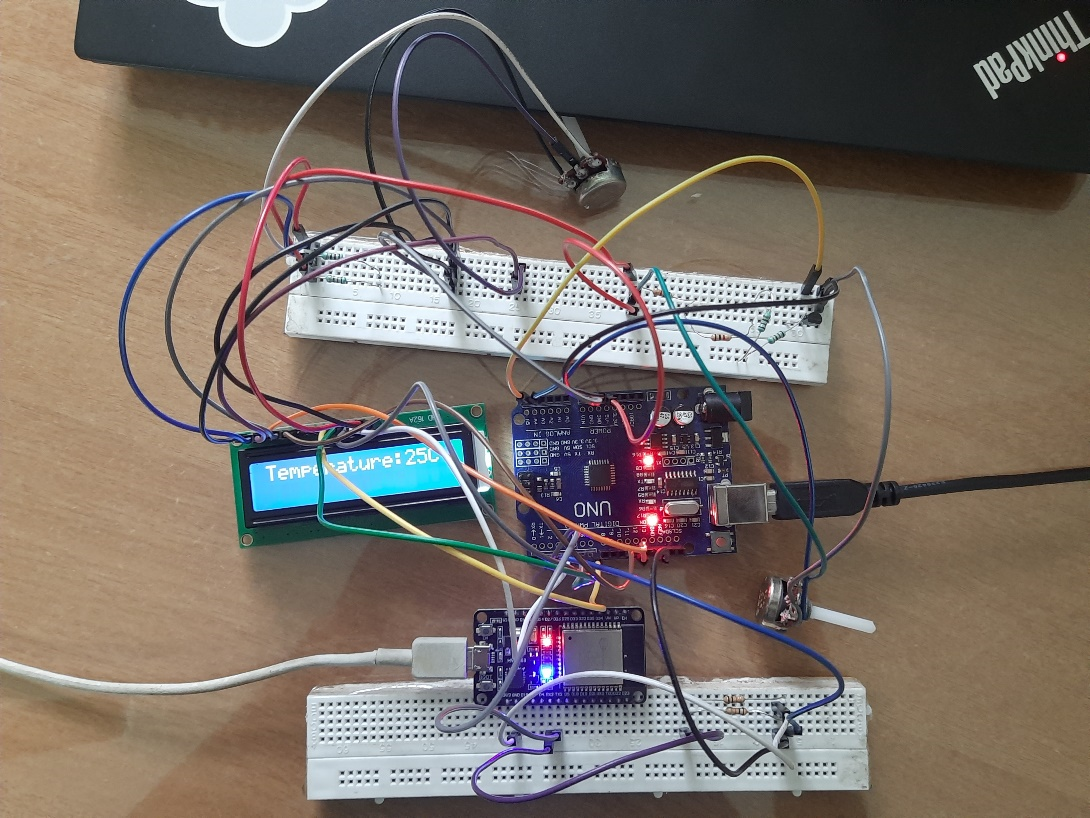
\includegraphics[width=\textwidth]{\LocTMPfig/project-setup.png}  \caption{Project Setup}
\end{figure}